% ============================================================
% Amazon-VT CFP 2026-2027 — 1-Page Abstract v4
% Proposal 3: Agentic Engineering Framework
% Primary: AI Accelerated Science & Engineering
% Secondary: Agentic AI
% Format: IEEE 2-column
% Revised: incorporates deep-research-topics.md insights
% ============================================================

\documentclass[conference, 10pt]{IEEEtran}

\usepackage[utf8]{inputenc}
\usepackage[T1]{fontenc}
\usepackage{graphicx}
\usepackage{hyperref}
\usepackage{microtype}
\usepackage{cite}
\usepackage{enumitem}
\setlist{nosep, leftmargin=1.5em, topsep=0.2em}
\usepackage{tikz}
\usetikzlibrary{positioning, arrows.meta, shapes.geometric, fit, calc}

\title{Agentic Knowledge Graphs for AI-Accelerated\\Engineering Across Domains}
\author{}
\date{}

% ============================================================
\begin{document}

\maketitle
\thispagestyle{empty}

\vspace{-1.5em}

\noindent\textbf{Primary Topic:} AI Accelerated Science \& Engineering \hfill
\textbf{Secondary:} Agentic AI

\vspace{0.5em}

AI-driven scientific breakthroughs---from biomolecular structure prediction~\cite{Abramson2024AlphaFold3} to materials discovery~\cite{Merchant2023GNoME}---demonstrate that domain-specific AI systems can dramatically accelerate discovery when tightly coupled to structured domain knowledge and simulation. Engineering disciplines face an analogous opportunity: construction, transportation, thermal systems, and manufacturing all involve domain-specific constraints, governing physical laws, simulation models, and structured design artifacts that must be reasoned over jointly. Yet large language models (LLMs) remain poorly suited to engineering: they hallucinate physical quantities~\cite{Ji2023HallucinationSurvey}, cannot enforce constraint satisfaction, and lack grounding in the structured ontologies and simulation feedback loops that define engineering practice. Meanwhile, physics-informed ML~\cite{Karniadakis2021PINN} and digital twin architectures~\cite{Tao2019DigitalTwin} have matured in isolation from generative AI, creating an integration gap between simulation-based engineering and the emerging agentic paradigm.

This project proposes \textbf{Agentic Knowledge Graph Engineering (AKG-E)}, a domain-agnostic framework that enables LLM-powered agents to reason over structured engineering knowledge, interact with physics-based simulations, and validate outputs against domain constraints. AKG-E provides three generalizable layers: (1)~a \textit{domain ontology layer} encoding engineering knowledge graphs with entities, constraints, physical laws, and design rules as pluggable, domain-specific components; (2)~a \textit{simulation integration layer} exposing domain simulation tools (e.g., FEniCS for PDE solving, IFC/BIM parsers for construction, traffic microsimulators) as agent-callable interfaces for simulation-in-the-loop validation; and (3)~a \textit{constraint validation layer} that automatically verifies agent-generated designs, analyses, and recommendations against physical and regulatory constraints before delivery. Agents orchestrate across these layers, selecting between retrieval-augmented generation~\cite{Lewis2020RAG}, structured graph queries~\cite{Edge2024GraphRAG}, and simulation calls based on task requirements and confidence.

\begin{figure}[t]
    \centering
    \resizebox{\columnwidth}{!}{%
    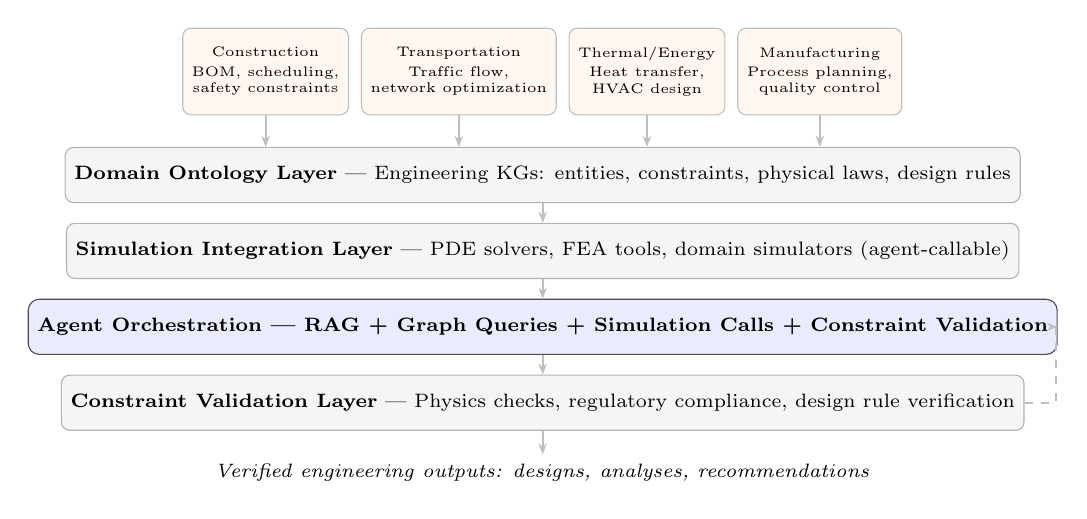
\begin{tikzpicture}[
        node distance=0.35cm and 0.25cm,
        layerbox/.style={rectangle, rounded corners=3pt, draw=gray!60, fill=gray!8, minimum width=7.5cm, minimum height=0.7cm, align=center, font=\scriptsize},
        dombox/.style={rectangle, rounded corners=3pt, draw=gray!50, fill=orange!6, minimum width=1.65cm, minimum height=1.1cm, align=center, font=\tiny},
        agentbox/.style={rectangle, rounded corners=4pt, draw=black!70, fill=blue!8, minimum width=7.5cm, minimum height=0.7cm, align=center, font=\scriptsize\bfseries},
        arr/.style={-{Stealth[length=4pt]}, thick, gray!50},
    ]
        % Domain applications (top)
        \node[dombox] (con) {Construction\\[1pt]\tiny BOM, scheduling,\\safety constraints};
        \node[dombox, right=0.15cm of con] (traf) {Transportation\\[1pt]\tiny Traffic flow,\\network optimization};
        \node[dombox, right=0.15cm of traf] (therm) {Thermal/Energy\\[1pt]\tiny Heat transfer,\\HVAC design};
        \node[dombox, right=0.15cm of therm] (mfg) {Manufacturing\\[1pt]\tiny Process planning,\\quality control};

        % Domain ontology layer
        \node[layerbox, below=0.4cm of $(con.south)!0.5!(mfg.south)$] (onto) {\textbf{Domain Ontology Layer} --- Engineering KGs: entities, constraints, physical laws, design rules};

        % Simulation integration layer
        \node[layerbox, below=0.25cm of onto] (sim) {\textbf{Simulation Integration Layer} --- PDE solvers, FEA tools, domain simulators (agent-callable)};

        % Agent orchestration
        \node[agentbox, below=0.25cm of sim] (agent) {Agent Orchestration --- RAG + Graph Queries + Simulation Calls + Constraint Validation};

        % Constraint validation
        \node[layerbox, below=0.25cm of agent] (val) {\textbf{Constraint Validation Layer} --- Physics checks, regulatory compliance, design rule verification};

        % Output
        \node[font=\scriptsize, below=0.3cm of val] (out) {\textit{Verified engineering outputs: designs, analyses, recommendations}};

        % Arrows
        \draw[arr] (con.south) -- (con.south |- onto.north);
        \draw[arr] (traf.south) -- (traf.south |- onto.north);
        \draw[arr] (therm.south) -- (therm.south |- onto.north);
        \draw[arr] (mfg.south) -- (mfg.south |- onto.north);
        \draw[arr] (onto) -- (sim);
        \draw[arr] (sim) -- (agent);
        \draw[arr] (agent) -- (val);
        \draw[arr] (val) -- (out);

        % Feedback loop
        \draw[arr, dashed] (val.east) -- ++(0.4,0) |- (agent.east);
    \end{tikzpicture}
    }%
    \caption{\textbf{AKG-E Framework.} Domain applications plug into a shared ontology layer. Agents orchestrate across structured retrieval, simulation interfaces, and constraint validation. A feedback loop ensures outputs satisfy physical and regulatory constraints. Domain-specific KGs and simulators are pluggable components; the orchestration and validation layers are domain-agnostic.}
    \label{fig:framework}
    \vspace{-0.5em}
\end{figure}

The key insight is that engineering problems share structural commonalities despite domain differences: a construction scheduling agent and a traffic optimization agent both require structured knowledge representation, agent-callable simulation interfaces, constraint enforcement, and provenance tracking~\cite{OpenTelemetryGenAI2024}. AKG-E abstracts these shared requirements into reusable layers while domain-specific knowledge graphs and simulators remain pluggable, yielding a \textit{generalizable method}---constraint-grounded agentic reasoning with simulation-in-the-loop validation---not merely a domain application.

This research investigates: (1)~how engineering domain ontologies can be represented as knowledge graphs that enable both LLM-based reasoning and structured constraint queries; (2)~how agents should orchestrate across retrieval, graph reasoning, and simulation calls to solve multi-step engineering problems; (3)~what simulation-in-the-loop validation mechanisms ensure agent outputs satisfy physical laws and domain constraints; and (4)~whether a domain-agnostic framework achieves competitive accuracy against domain-specific systems while reducing development cost.

We will demonstrate AKG-E in \textbf{construction planning} (BOM reasoning, structural verification via FEA) and \textbf{transportation systems} (traffic flow optimization via digital twin simulation), with thermal engineering as an extension domain. Agents invoke domain simulators, validate outputs against physical and regulatory constraints, and update digital twin state. Measurable targets include constraint violation reduction and decision accuracy vs.\ expert baselines. Experiments compare prompt-only LLMs, RAG-augmented methods, and the full AKG-E framework. Expected outcomes include the open AKG-E framework, pluggable engineering KG templates, and benchmarks demonstrating that \textbf{simulation-grounded agentic AI} outperforms unstructured approaches for engineering decision-support.

\bibliographystyle{IEEEtran}
\bibliography{references}

\end{document}
